\section{Introduction}
\label{introduction}
\todo{Introduction}

There exist 2 equivalent interpretations of the Lonely Runner conjecture that are widely used:\todo{have a footnote where it was named}
\begin{enumerate}
\item Imagine $n$ runners at a circular, unit length track\footnote{I.E. the track has a circumference of 1}, where every runner runs with a constant, pairwise different speeds\footnote{These speeds can, without loss of generality be assumed to be in $\N$ \cite{Bienia97flows.view-obstructions} - also see \ref{integerSpeeds}}, there will then be a time when all runners will be at least $\frac{1}{n + 1}$ units away from their common start-point.\\

\item Alternatively, imagine that we instead have n + 1 runners, then the conjecture states that there exists a point in time where all the runners are at least $\frac{1}{n + 1}$ units away from their nearest runner. Everything else is the same as in the first interpretation \cite{Bienia97flows.view-obstructions}.\\
\end{enumerate}

More formally the problem can be stated thus: 
Given any n positive integers $w_1, w_2, \ldots, w_n$, there is a real number $x$ such that 
\eqn{
\label{eqa:lonelyRunner} \Vert w_i x\Vert \geq \frac{1}{n+1}
}

for each $i = 1, 2, \ldots, n$, where for a real number $y$, $\Vert y \Vert$ is the distance from $x$ from the nearest integer. I owe this formulation of the problem to \cite{ANote}.

\subsection{Expectations to the reader}
\label{expectations}
\todo{Expectations}
I expect the reader to be able to understand the Lonely Runner Conjecture in all its formulations, as well as being mathematically mature, and having a basic understanding of Plane Sweep algorithms.

\subsection{Scope and Limitations}
\label{scope}
\todo{Scope and limitations}
\begin{itemize}
\item In this project I will not attempt to prove the Lonely Runner conjecture for all n. 
\item I will work to make the program return a result within a reasonable time, for up to 1000 runners, and with speeds up to 1000. The final program should work with more than 1000 runners, and with speeds in excess to 1000, but I will not optimise it further. 
\item The program will include an interactive counterexample search system.
\item I will only focus on runners with integer speeds - see \ref{integerSpeeds} for an justification of this.
\end{itemize}

\subsection{Integer speeds}
In this section I will argue that I need only focus on integer speeds.
Let us assume there is a non-empty set S of runner speeds that are not integers. Since we are dealing with the speeds of runners, it is clear that it only makes sense either all elements in S belong to $\mathbb{Q}$ or where at least one of the elements in S is a irrational number:
\begin{description}
\item[Only rational numbers in S:] In this instance we can convert all the runner speeds into integers, by multiplying all speeds (also those not in S) with the product of the denominators, of all the rational numbers in S.
\item[Irrational numbers exist in S:]   
\end{description}

\subsection{Terminology}
\label{Termonolgy}
\begin{figure}[H]
  \centering
  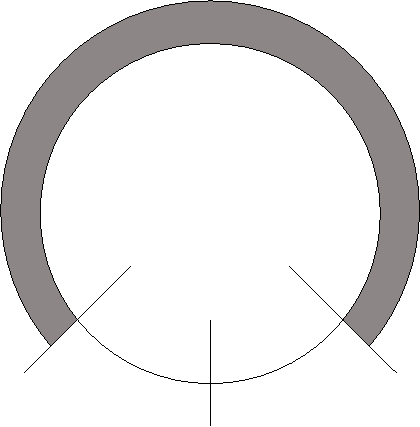
\includegraphics[width=0.3\textwidth]{./images/circleZonePng.png}
  \caption{\label{circleZoneImg}An illustration of the Runner track. The grayed out part is the Zone}
\end{figure}

In this report I will refer to the track interval [$\frac{1}{n + 1}$, $\frac{n}{n+1}$] as the Zone, and a runner who is in this interval, as ``being in the Zone''.

When forced to use a pronoun by the English language, I will use the male pronoun to the refer to the runners. This is done purely for convenience, and to make the text flow better. Not because I believe that male runners are more numerous or in any way inherently better than female runners.

Configurations of runners, will in this report refer to a set S of $n \in \N$ runners, where for all runners $r \in S$, $r_{speed} \in \N$, and $r\prime_{speed} \neq r_{speed}$ where $r\prime \in S \setminus r$.

When talking about the fake runner, I will be referring to a runner that is not actually in race (or any attempt to find a value that would make the Lonely Runner conjecture valid for the given configuration of runners), but rather a runner that has been introduced for convince.   

\subsection{Background material used}
\label{background}
For this project I have read the following papers dealing with the Lonely Runner conjecture: ``View-Obstruction Problems''\cite{Bienia97flows.view-obstructions}, ``The lonely runner problem with seven runners'' \cite{serra_thelonely}, ``Regular chromatic number and the lonely runner problem'' \cite{Barajas2007479}, ``View-Obstruction Problems'' \cite{springerlink:10.1007/BF01832623}, ``Tight Instances of the Lonely Runner'' \cite{Goddyn96tightinstances}, ``A Note on the Lonely Runner Conjecture'' \cite{ANote} and ``Invisible runners in finite fields'' \cite{invis}.

I have also used the follow support literature:
``Computational Geometry'' \cite{citeulike:3347056}, ``Uniform Distribution of Sequences'' \cite{uniform} and ``Kalkulus'' \cite{kalkulus}.

\subsection{Overview}
\todo{Make sure overview fits with the actual content}

In this section I give a quick overview of what the different sections in report will cover.
\begin{description}
\item[Section \ref{introduction}] The introduction to the report, which will introduce the subject and explain my goals
\item[Section \ref{choiceOfMethod}] A discussion of the two different approaches that can decide whether or not the Lonely Runner conjecture holds for a given configuration
\item[Section \ref{implementation}] Description of the implementation details and an analysis of the scalability of the implementation
\item[Section \ref{test}] The test results
\item[Section \ref{results}] Interpretation of results
\item[Section \ref{conclusion}] The conclusion of the report  
\end{description}
